\documentclass{article}
\usepackage{tikz}
\usetikzlibrary{angles, backgrounds, calc}

\tikzset{
  dot/.style={
    circle, fill=black, inner sep=1pt, outer sep=0pt
  },
  dot label/.style={
    circle, inner sep=0pt, outer sep=1pt
  },
  % act on every pics named "right angle"
  pics/right angle/.append style={
    /tikz/draw, /tikz/angle radius=5pt
  }
}


\begin{document}

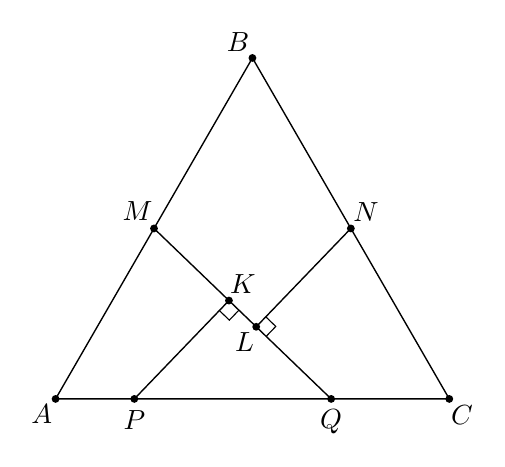
\begin{tikzpicture}
  % denote absolute points
  \path coordinate (A) at (0, 0) 
        coordinate (B) at (60:5)
        coordinate (C) at (5, 0);
  % denote relative points
  \path coordinate (M) at ($ (A)!.5!(B) $)
        coordinate (N) at ($ (B)!.5!(C) $)
        coordinate (Q) at ($ (C)!.3!(A) $)
        coordinate (P) at ($ (C)!.8!(A) $)
        coordinate (K) at ($ (M)!(P)!(Q) $)
        coordinate (L) at ($ (M)!(N)!(Q) $);
  % draw lines
  \draw[line width=.5pt] 
    (A) -- (B) -- (C) -- cycle 
    (M) -- (Q)
    (P) -- (K)
    (N) -- (L);
  % mark right angles
  \draw pic {right angle=P--K--Q}
        pic {right angle=N--L--Q};
  % mark points
  \foreach \i/\angle in {A/-120, B/120, C/-80, M/120, N/60, P/-90, Q/-90, K/80, L/-95} {
    \node[dot, label={[dot label]\angle:$\i$}] at (\i) {};
  }
\end{tikzpicture}
\bigskip


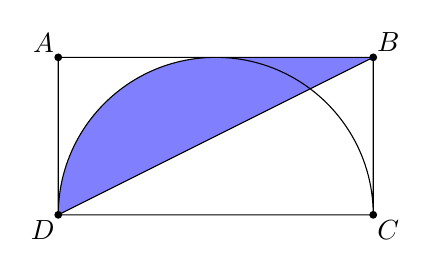
\begin{tikzpicture}[scale=2]
  % denote absolute points
  \path (0, 0) coordinate (D)
        (2, 1) coordinate (B);
  % denote relative points
  \path (D -| B) coordinate (C)
        (D |- B) coordinate (A);
  % mark points
  \foreach \i/\angle in {A/135, B/45, C/-45, D/-135} {
    \node[dot, label={[dot label]\angle:$\i$}] at (\i) {};
  }
  % draw lines and arc
  \draw (D) rectangle (B)
        (D) -- (B)
        (C) arc[start angle=0, end angle=180, radius=1];
  % fill region
  \begin{scope}[on background layer]
    \fill[fill=blue!50, line join=bevel] (D) -- (B) -- ($ (B)!.5!(A) $) arc[start angle=90, end angle=180, radius=1] -- cycle;
  \end{scope}
\end{tikzpicture}
\end{document}
